%!TEX root = thesis.tex
\chapter{Background}
\label{cha:background}

Linguistics --- the scientific study of human language --- has investigated the way in which humans acquire language, how they develop and refine their linguistic capabilities and how they apply what they have learnt. Within the field of linguistics, it is widely accepted that language is a key component in establishing mental models, which allow humans to reason about how something works as well as define and communicate their approach to solving problems \cite{Johnson86a}.

When building software, developers write source code in a programming language that can be understood and executed by the device for which it was intended. However, in order to facilitate communication with other developers, modern programming languages allow developers to name the symbols that make up a program using words that they are familiar with that are of semantic relevance to the itself. It is these symbol names that are embedded within the source code, as opposed to the selection of programming language, that is the most important facet in the development of a mental model of a software system. By utilising a collection of semantically rich terminology within the source code, developers are able to establish a shared vocabulary that is representative of the software's domain and architecture, which is useful in facilitating program comprehension.

Studies of natural language have shown that a person's vocabulary continues to grow throughout their lifetime, but that the amount of words that one can include in their vocabulary is only a subset of all the words in a language \cite{Nation93a}. Furthermore, when practically applied in writing natural language documents, a person tends to heavily favour the use of a small number of terms in their vocabulary and use the rest only sparingly \cite{Zipf49a}.

A natural question that arises in this context is: \emph{Do symbol names (vocabulary) created to represent software solutions exhibit similar properties and how do they evolve?}

In this chapter, we explore the current understanding of vocabularies in software and how the effects that evolution has upon them. In doing so, we highlight some of the current gaps in knowledge within the literature, and motivate our own research questions.

The chapter is structured as follows:

\textbf{\secref{vocabulary} - Vocabulary} describes vocabularies, the role that they play and how they are built and evolved.

\textbf{\secref{source_code_vocabulary} - Source Code Vocabulary} highlights the differences in natural language and source code vocabularies and the research efforts to establish a vocabulary for developers.

\textbf{\secref{mental_models} - Mental Models} discusses the role of mental models in problem solving, their ability to adapt to change and the importance of a shared mental model within teams.

\textbf{\secref{software_mental_models} - Software Mental Models} outlines how mental models relate to software development, the difficulty of building a software mental model and research that has looked to improve development of mental models for software.

\textbf{\secref{source_code_vocabulary_evolution} - Source Code Vocabulary Evolution} presents the current understanding of the effects of software evolution on source code vocabularies.

\section{Vocabulary} % (fold)
\label{sec:vocabulary}

Vocabulary describes the set of words within a language a person knows and is able to use \cite{Woodford03a}. The purpose of building a vocabulary is to facilitate a person's comprehension of the things that they encounter and allow them to be expressive in communicating these ideas. A vocabulary usually grows and evolves with age as humans are exposed to new things are learn new ways to describe things that they had previously encountered \cite{Wren00a}. This allows them to become more precise in the language that they associate with something.

Humans, when in their stages of infancy, are able to acquire new vocabulary through words that they hear used by others that associate with their surroundings \cite{Gathercole92a}. Through continued exposure to this, they are then able to use the words that they have acquired to express themselves effectively. During this stage of development, the growth of vocabulary is relatively unhindered and thus humans are able to acquire new words at a high rate \cite{Metsala98a}. As the development of vocabulary becomes more sophisticated, through exposure to reading and writing, there is an inherent complexity brought about by the relationships formed between words in the vocabulary and how they can be meaningfully applied \cite{Dickinson03a}. This decreases the rate at which new information can be augmented into an existing vocabulary \cite{Fisher94a}.

Due to the sheer volume of terms that there are in any natural language, it is beyond the capacity of most humans to know and be able to use every word that exists  within a language. Typically, the vocabulary size of a college-educated person ranges between 12,000--17,000 words \cite{Zechmeister95a}. As a consequence of this, the brain will prioritise the recall of terms that are of the highest importance and most frequent practical use. While vocabularies are flexible to change based on the needs of an individual, the magnitude of change impacts the ability of vocabularies to be augmented to incorporate new information.

Despite the fact that vocabularies grow to accommodate such a large number of terms, when vocabulary is applied in writing a natural language document, the number of terms used is significantly less than the total size of the vocabulary \cite{Biber98a}. Furthermore, the majority of terms used within a natural language document occur only a small number of times (see \figref{vocab_freqdist_gadfly}). Typically, the most frequently used terms are conjunctive words (\eg \emph{and}, \emph{or}, \emph{for}, etc.), while the use of other language is context-specific \cite{McEnery01a}.

\begin{figure}[t]
\centering
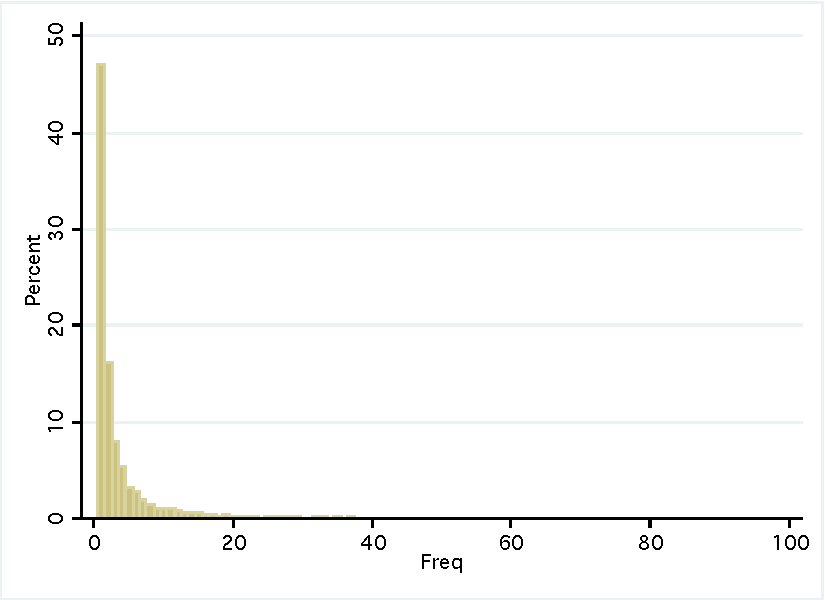
\includegraphics[width=\textwidth]{Figures/Vocab-GadflyFreqDist.pdf}
\caption{Term frequency distribution for \emph{The Gadfly} by Ethel Lilian Voynich, 1897, showing a preference towards using a large percentage of terms infrequently}
\label{fig:vocab_freqdist_gadfly}
\end{figure}

% section vocabulary (end)

\section{Source Code Vocabulary} % (fold)
\label{sec:source_code_vocabulary}

When writing source code, there are very few limitations placed on developers in regard to the elements of their vocabulary they are able to use in their source code; the only limitation being the need to conform to the rules of the platform that the code is intended for. Because of this, developers are able to utilise their vocabulary to express intent within the source code. However, the guidelines as to how developers apply vocabulary appropriately within source code are not well defined.

In contrast to natural language vocabularies that are refined through application in writing documents, developers get little exposure to and feedback on how to use language effectively within their code. As a result, developers are required to adapt their understanding of how to use vocabulary to write code, which is fundamentally different from natural language \cite{Naur75a}.

Despite the fundamental differences between natural language and source code, studies that have compared the application of vocabulary within source code \cite{Pierret09a, Delorey09a} have found that there is a skewed distribution for term usage within source code that is similar to that found in natural language documents. Abebe \etal \cite{Abebe09a} investigated the most frequently used terms in ALICE\footnote{ALICE (A Large Ion Collider Experiment) \url{http://www.alice.org/}} and WinMerge,\footnote{WinMerge differencing and merging tool \url{http://winmerge.org/}} finding that domain-related terminology was amongst the most popularly used terms for both systems.

Recent studies by H{\o}st and {\O}stvold \cite{Host07b, Host09a} have investigated the vocabulary used by developers within the source code of Java projects to determine if there are common usage patterns for terminology. \cite{Host07b} focused on the way in which developers use verbs within their code based on the behavioural characteristics of functions containing a particular verb within their name. Their study produced \emph{The Programmer's Lexicon}, which describes a number of commonly found terms within function names and the kind of behaviour typically associated with the terms; the purpose of which was to identify and vocabulary usage already established by Java programmers. H{\o}st and {\O}stvold built upon this work \cite{Host09a} by characterising combinations of parts of speech to determine the grammatical structure of method names and the meaning of the phrases as commonly used by Java programmers.

These studies have given an insight into how developers apply vocabularies within their source code and have shown that there are commonalities across project in regard to how terms are used to characterise behaviour. However, the studies do not describe the effects of developer's choices in their use of vocabulary, whether it is appropriate in facilitating program comprehension and how this effects the ability of a system to evolve.

% section source_code_vocabulary (end)

\section{Mental Models} % (fold)
\label{sec:mental_models}

Mental models describe the cognitive processes of humans in being able to comprehend things that they are exposed to \cite{Gentner83a}. They allows us to develop an understanding of something that is akin to our usual patterns of thought, which in turn, makes it easier and more natural to reason about \cite{Johnson86a}. The establishment and subsequent application of a mental model is relevant in the context of problem solving, as it helps define an approach to finding a solution to problems \cite{Johnson86a}.

Development of a mental model is particularly important when dealing with complex problems, as it allows us to break down complexity such that it can be managed effectively \cite{Johnson86a}. This in turn enables us to be more productive in solving a problem through smaller and more focused efforts.

While mental models are built by individuals as a means of comprehension, representative mental models are also built amongst members of a team tasked to solved a problem, through a shared understanding of what the problem and its solution entails \cite{Mathieu00a}. Finding a solution to complex problems can often entail unconventional thinking in order to reveal a solution that may be masked by the complexity inherent within the problem. However, the involvement of more than one individual requires some degree of alignment in the mental models of those involved such that they are able to work towards a common goal \cite{Lim06a}.

Once a mental model has been built, it is able to adapt to changes in the environment or circumstances in which it was initially established. However, mental models can become resistant to change in when they become too ingrained as part of an individuals understanding of something \cite{Johnson86a}; a problem which is magnified when the mental model is shared within a team \cite{Lim06a}.

Languages play a significant role in building mental models, as we as humans associate our comprehension of something with the language we have acquired that can be used to describe it \cite{Fauconnier94a}. Therefore, a shared mental model requires a vocabulary that is consistently understood and applied.

% section mental_models (end)

\section{Software Mental Models} % (fold)
\label{sec:software_mental_models}

Software systems are complex entities that require that their users have an understanding of the problem that the software is trying to solve and how it will enable them to solve it. In order to do this, users will build a mental model of how the software works in order to use it effectively \cite{Carroll87a}. To ease the development of mental models for users, there is a responsibility on the part of the developers to ensure the software is not overly complex \cite{Krug05a}.

Developers must also form a mental model of the software when they are building it \cite{Storey99a}. This allows them to not only translate the requirements outlined by the problems that they intend the software to solve into a functional solution, but also to construct the software such that it is maintainable and extensible \cite{Littman87a}.

Unfortunately, developing software is considerably more abstract than, say, building a house. As a result, obtaining an understanding of a problem and translating it into a viable solution is rarely straightforward \cite{Leffingwell99a}. This makes it difficult to establish a mental model of the software as a basis for its implementation \cite{Storey99a}.

Developers have the responsibly of not only understanding how the software works, but also to communicate to a computer how it should behave and to other developers how it is constructed \cite{Abelson96a}. Fortunately, developers are able to rely heavily on real-world concepts as metaphors in communicating to other developers how a software system has been built. The use of the object-oriented programming paradigm \cite{Wirfs90a} and design patterns \cite{Gamma95a} have allowed a cognitive map for developers to apply traditional thinking within a software context. While these concepts are applicable across most kinds of software system, the lack the specificity that is required for program comprehension. To account for this, developers require a set of domain-specific abstractions that can be used to provide a better understanding of the systems they are building.

Biggerstaff \etal \cite{Biggerstaff93a} pioneered efforts into understanding how human-oriented concepts can be mapped to implementation-oriented concepts within software systems. In their study, they found that direct links between the two are hard to establish and priori knowledge is required to make such an inference.

Studies of the relationship between mental models and the language used by developers have primarily focused on the impact of identifier\footnote{Identifiers are tokens which name language entities} quality on program 
comprehension \cite{Takang96a,Anquetil98a,Caprile99a,Maletic01a,Deissenboeck06a,Rilling03a,Caprile00a,Lawrie06a,Lawrie06b,Lawrie07a} and improving the quality of identifiers that developers use \cite{Deissenboeck06a,Lawrie07a,Caprile99a,Caprile00a, Abebe09b}.

Dei{\ss}enb\"{o}eck and Pizka \cite{Deissenboeck06a} proposed rules for well-formed identifiers based on two characteristics: \emph{conciseness} and \emph{consistency}. In their study they built an \emph{identifier dictionary} describing each of the terms found within symbol names for the systems that were analysed, which allowed them to detect when the rules had been violated. Lawrie \etal \cite{Lawrie07a} performed an empirical study of these rules based on two case studies, which showed that developers frequently violated the rules in their naming their identifiers.

Lawrie \etal \cite{Lawrie06a} examined the impact of identifier completeness upon the comprehension of developers. In their study, they assess the ability of over 100 developers to comprehend function identifiers at three different levels of completeness --- \emph{single letters}, \emph{abbreviations}, and \emph{full words} --- based on well-known algorithms and production code samples. Their study showed that full word identifiers lead to the highest level of comprehension, although in a lot of cases the difference between abbreviation and full word identifiers was negligible.

Abebe \etal \cite{Abebe09b} classified ``bad smells'' in the identifiers written by programmers that could potentially diminish the program comprehension abilities of those working with the software. Their study outlined how these bad smells could be detected and subsequently removed in order to allow for greater readability and comprehension.

These studies have demonstrated that the language used by developers is important in facilitating program comprehension required for development and subsequent maintenance of software systems. However, they have not provided much insight into how the collection of terms forming the vocabulary is used within source code and how this changes as the software evolves.

% section software_mental_models (end)

\section{Source Code Vocabulary Evolution} % (fold)
\label{sec:source_code_vocabulary_evolution}

Research efforts to investigate the effect of software evolution upon the vocabulary used by developers has so far been limited. Primarily they have focused upon the evolution of a system's vocabulary compared to the system itself.

Antoniol \etal \cite{Antoniol07a} assessed the stability of the source code lexicon\footnote{Lexicon is a language's vocabulary, including its words and expressions} compared to the stability of program structure through evolution of Mozilla,\footnote{Mozilla browser (Firefox) \url{http://www.mozilla.com/firefox}} ALICE and Eclipse.\footnote{Eclipse IDE \url{http://www.eclipse.org/}} Their study found that both the lexicon and program structure evolved towards higher stability, though the lexicon was more stable overall. Interestingly, they found that the lexicon and program structure showed similar patterns in evolution. Their study also looked at the amount of change that occurred in program entities due to identifier refactoring, finding that changes to the lexicon were rare. They argued that the stability of the lexicon in the systems they analysed indicated that developers had formed a mental model that would be costly change.

Abebe \etal \cite{Abebe09a} analysed the evolution of vocabulary for ALICE and WinMerge. Their study found that the size of the vocabulary and the size of a software system tend to evolve in the same way and that the vocabulary used in comments has a higher rate of growth than vocabulary that is used within executable parts of the code. Their study also found that the creation of new identifiers typically did not introduce new terms, indicating that developers re-use existing terms.

While these studies have allowed some insight into how evolution affects the vocabulary used by developers, they have been limited in terms of the number of systems and diversity of systems investigated. Hence, there is insufficient evidence to be able to generalise across software systems.

% section source_code_vocabulary_evolution (end)

\section{Research Questions} % (fold)
\label{sec:research_questions}

Research investigating how humans use natural language and build vocabularies have found that a rich vocabulary of terms is important in building mental models used to solve problems. However, while we have formed some idea of how natural language vocabularies are established and evolved, we know little about how they are utilised within source code and the impact that evolution has upon the vocabulary of developers.

In order to address the gaps identified, we framed a set of research questions related to the evolutionary properties of source code vocabularies.

The questions that we address in this thesis are as follows:
\vspace{-0.28cm} %% formatting on the same page
\begin{itemize}
	\item How do source code vocabularies grow throughout evolution? Does the rate of growth for vocabulary match the rate of growth for system size?
	\item What is the frequency of usage distribution for terms in a source code vocabulary? Does this match that which can be found in natural language documents?
	\item What do the most frequently used terms refer to? Can we mine the domain model from a system using the most frequently used terms?
	\item How does the distribution of terms change across releases? Are frequently used terms continually re-used? Are changes to the distribution stable or erratic?
	\item Does the age of a term dictate its likelihood of being re-used?
\end{itemize}

The next chapter (\chapref{method}) presents the input data set, how we selected systems for our investigation and how we extracted vocabularies from the source code. \chapref{findings} outlines our method of analysis and the key findings that are resultant from investigation. The implications of our findings are discussed in \chapref{implications} and \chapref{conclusions} concludes the thesis.

% section research_questions (end)

% chapter background (end)